\documentclass{article}
\usepackage[left=3cm, right=3cm, top=3cm, bottom=3cm]{geometry}
\usepackage{graphicx}

\begin{document}

\begin{center}
	\vspace*{100px}
	\Huge Data Mining And Warehousing \\
	\vspace{60px}
	\LARGE \textbf{Mini Project: Diabetes prediction on Pima Indian Diabetes dataset.}\\
	\vspace{100px}
	\textit{Aanshi Verma}  (422068) \\
	\textit{Krishna Purohit} (422030) \\
	\textit {Akash Varma} (423064) \\
\end{center}
\newpage
\normalsize

\section{Objective}

Consider a labelled dataset belonging to an application domain. Apply suitable data preprocessing steps such as handling of null values, data reduction, descretization. For prediction of class labels of given data instances, build classifier models using different techniques (minimum 3), analyze the confusion matrix and compare these models. Also apply cross validation while preparing training and testing datasets.


\section{Introduction}

For the purpose of this project, we have decided to use healthcare related data to perform classification. We will use Pima-Indian diabetes dataset for the purpose of supervised classification of patients on the basis of their medical history and checkup reports.

\par Diabetes means blood sugar is above desired level on a sustained basis. The prime objective of this research work is to provide a better classification of  diabetes. There are already several existing method, which have been implemented for the classification of  diabetes dataset. In medical sector, the classifications systems have been widely used to exploit the patient’s data and make the predictive models or build set of  rules. In this manuscript firstly Naive Bayes used for the classification on all the attributes and then genetic algorithms used as an attribute selection and Naive Bayes used on that selected attribute for classification. The experimental results show the performance of  this work on Pima Indian Diabetes Dataset (PIDD) and provide better classification for diagnosis.

\section{Dataset}

\textbf{Origin:} The dataset is collected from a tribe of native Americans called `Pima'. Pima are a group of Native Americans living in an area consisting of what is now central and southern Arizona. The majority population of the surviving two bands of the Akimel O'odham are based in two reservations: the Keli Akimel O'otham on the Gila River Indian Community (GRIC) and the On'k Akimel O'odham on the Salt River Pima-Maricopa Indian Community (SRPMIC).
\par In the recent years, because of a sudden shift from traditional agricultural crops to processed foods, together with a decline in physical activity, made them develop the highest prevalence of type 2 diabetes and for this reason they have been subject of many studies.
\par The dataset includes data from 768 women with 8 characteristics, in particular:
\begin{enumerate}
	\item Number of times pregnant
	\item Plasma glucose concentration a 2 hours in an oral glucose tolerance test
	\item Diastolic blood pressure (mm Hg)
	\item Triceps skin fold thickness (mm)
	\item 2-Hour serum insulin (mu U/ml)
	\item Body mass index (weight in kg/(height in m)\textasciicircum2)
	\item Diabetes pedigree function
	\item Age (years)
\end{enumerate}
The last column of the dataset is the outcome of the study, which shows whether the person has diabetes or not (represented by 0 for negative and 1 for positive), which we will use for the purpose of classification.

\par The type of dataset and problem is a classic supervised binary classification. Given a number of elements all with certain characteristics (features), we want to build a machine learning model to identify people affected by type 2 diabetes.

To solve the problem we will have to analyse the data, do any required transformation and normalisation, apply a machine learning algorithm, train a model, check the performance of the trained model and iterate with other algorithms until we find the most performant for our type of dataset.


\section{Proposed methodology}

For this project, we have proposed the following workflow as represented by the following block diagam (figure 1).
The  block  diagram  of   proposed  approach  is  shown  above  and  next  proposed  approach  is  as  follows:
\begin{enumerate}
	\item Download the PIDD dataset from UCI machine learning repository or kaggle.com
	\item Load the dataset into a dataframe (use pandas library in python)	
	\item Preprocess the data
	\begin{itemize}
		\item Remove NaN values
		\item Normalize the data
	\end{itemize}
	\item Split the data into training and testing datasets using cross-validation
	\item Train various models
	\item Test the accuracy of all models using test dataset
	\item Compare the accuracy of all models and analyze the results
\end{enumerate}
	
\begin{figure}[h]
	\centering
	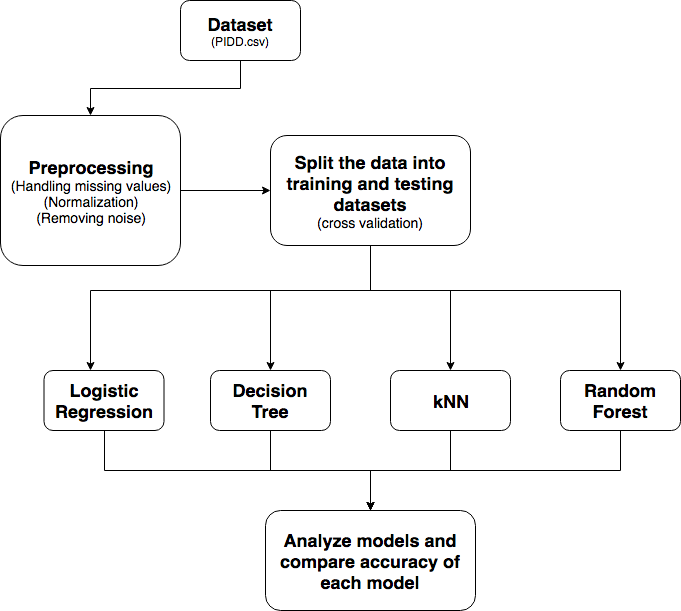
\includegraphics[width=280px]{workflow.png}
	\caption{workflow}
\end{figure}


\section{Algorithms}
\begin{enumerate}
	\large \item \textbf{kNN (k-nearest neighbors)}
	\normalsize
	\par In pattern recognition, the k-nearest neighbors algorithm (k-NN) is a non-parametric method used for classification and regression. In both cases, the input consists of the k closest training examples in the feature space. The output depends on whether k-NN is used for classification or regression: 
	\begin{itemize} 
		\item In k-NN classification, the output is a class membership. An object is classified by a majority vote of its neighbors, with the object being assigned to the class most common among its k nearest neighbors (k is a positive integer, typically small). If k = 1, then the object is simply assigned to the class of that single nearest neighbor.
		\item In k-NN regression, the output is the property value for the object. This value is the average of the values of its k nearest neighbors.
	\end{itemize}
	\par k-NN is a type of instance-based learning, or lazy learning, where the function is only approximated locally and all computation is deferred until classification. The k-NN algorithm is among the simplest of all machine learning algorithms. Both for classification and regression, a useful technique can be used to assign weight to the contributions of the neighbors, so that the nearer neighbors contribute more to the average than the more distant ones. For example, a common weighting scheme consists in giving each neighbor a weight of 1/d, where d is the distance to the neighbors.
	
	\begin{figure}[h]
		\centering
		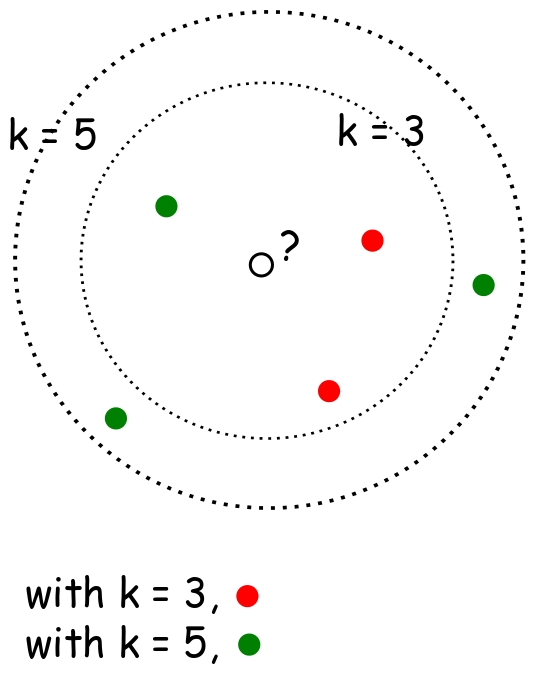
\includegraphics[width=200px]{knn.png}
		\caption{illustration of kNN}
	\end{figure}

	The training examples are vectors in a multidimensional feature space, each with a class label. The training phase of the algorithm consists only of storing the feature vectors and class labels of the training samples.

	In the classification phase, k is a user-defined constant, and an unlabeled vector (a query or test point) is classified by assigning the label which is most frequent among the k training samples nearest to that query point.

	A commonly used distance metric for continuous variables is Euclidean distance. For discrete variables, such as for text classification, another metric can be used, such as the overlap metric (or Hamming distance). In the context of gene expression microarray data, for example, k-NN has also been employed with correlation coefficients such as Pearson and Spearman. Often, the classification accuracy of k-NN can be improved significantly if the distance metric is learned with specialized algorithms such as Large Margin Nearest Neighbor or Neighbourhood components analysis.

	A drawback of the basic ``majority voting" classification occurs when the class distribution is skewed. That is, examples of a more frequent class tend to dominate the prediction of the new example, because they tend to be common among the k nearest neighbors due to their large number. One way to overcome this problem is to weight the classification, taking into account the distance from the test point to each of its k nearest neighbors. The class (or value, in regression problems) of each of the k nearest points is multiplied by a weight proportional to the inverse of the distance from that point to the test point. Another way to overcome skew is by abstraction in data representation.
	\vspace{10px}
	\large \item \textbf{Logistic Regression}
	\normalsize 
	\par Logistic regression is the appropriate regression analysis to conduct when the dependent variable is dichotomous (binary).  Like all regression analyses, the logistic regression is a predictive analysis.  Logistic regression is used to describe data and to explain the relationship between one dependent binary variable and one or more nominal, ordinal, interval or ratio-level independent variables.
	\par In statistics, the logistic model (or logit model) is a widely used statistical model that, in its basic form, uses a logistic function to model a binary dependent variable; many more complex extensions exist. In regression analysis, logistic regression (or logit regression) is estimating the parameters of a logistic model; it is a form of binomial regression. Mathematically, a binary logistic model has a dependent variable with two possible values, such as pass/fail, win/lose, alive/dead or healthy/sick; these are represented by an indicator variable, where the two values are labeled "0" and "1".	
	\par An explanation of logistic regression can begin with an explanation of standard logistic function. The logistic function is a sigmoid function, which takes any real input \textit{t} (\textit{t} $\in$ \textit{R}), and outputs a value between zero and one; for the logit, this is interpreted as taking input log-odds and having output probability. The most widely used formula for standard logistic regression is:
	
	\[f(x) = \frac{1}{1 + e^{-x}} = \frac{e^{x}}{e^{x} + 1}\]
	
	\begin{figure}[t]
		\centering
		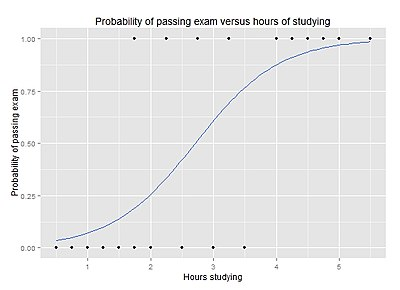
\includegraphics[width=400px]{logistic.jpg}
		\caption{logistic curve}
	\end{figure}
	
	\newpage
	\vspace{10px}
	\large \item \textbf{ Decision Tree}
	\normalsize
	\par A decision tree is a decision support tool that uses a tree-like graph or model of decisions and their possible consequences, including chance event outcomes, resource costs, and utility. It is one way to display an algorithm that only contains conditional control statements. Decision trees are commonly used in operations research, specifically in decision analysis, to help identify a strategy most likely to reach a goal, but are also a popular tool in machine learning.
	
	\textbf{Decision tree learning : } Decision tree learning uses a decision tree (as a predictive model) to go from observations about an item (represented in the branches) to conclusions about the item's target value (represented in the leaves). It is one of the predictive modelling approaches used in statistics, data mining and machine learning. Tree models where the target variable can take a discrete set of values are called classification trees; in these tree structures, leaves represent class labels and branches represent conjunctions of features that lead to those class labels. Decision trees where the target variable can take continuous values (typically real numbers) are called regression trees. In decision analysis, a decision tree can be used to visually and explicitly represent decisions and decision making. In data mining, a decision tree describes data (but the resulting classification tree can be an input for decision making). This page deals with decision trees in data mining.
	
	\begin{figure}[h]
		\centering
		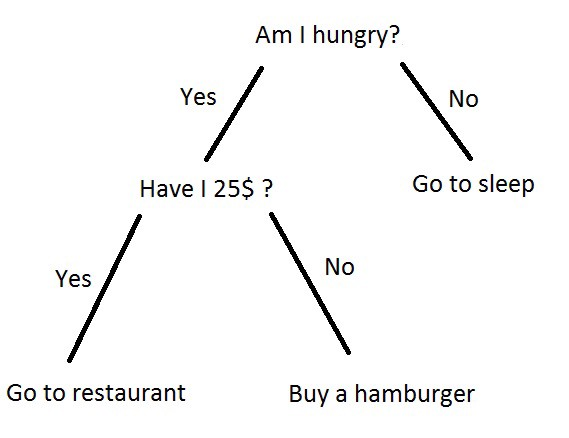
\includegraphics[width=200px]{decision_tree.jpg}
		\caption{decision tree}
	\end{figure}
	
	Decision trees used in data mining are of two main types: 
	\begin{itemize}
		\item \textbf{Classification tree} analysis is when the predicted outcome is the class to which the data belongs.
		\item \textbf{Regression tree} analysis is when the predicted outcome can be a real number (eg. the price of a house, or a patient's length of stay in a hospital).
	\end{itemize}

	There are many specific decision-tree algorithms. Notable ones include:
	\begin{itemize}
		\item ID3 (Iterative Dichotomiser 3)
		\item C4.5 (successor of ID3)
		\item CART (classification and regression tree)
		\item CHAID (Chi-squared Automatic Interaction Detector)
	\end{itemize}
	\par Decision trees use entropy to find out the best root of the tree, i.e. the node which gives us the most `information' about the dataset. In particular, most widely used concept is the Shannon's entropy formula, which is iteratively used to identify which column or input gives the most information about the output in dataset.
	\[H(X) = E[I(X)] = E[-\log(P(X)) ]\]
	The entropy can be explicitly written as:
	\[ \sum_{i=1}^{n} P(x_{i}I(x_{i})) = -\sum_{i=1}^{n}P(x_{i})\log_{b}P(x_{i}) \]
	
	
	\vspace{10px}	
	\large \item \textbf{ Random Forest}
	\normalsize	
	
	\begin{figure}[h]
		\centering
		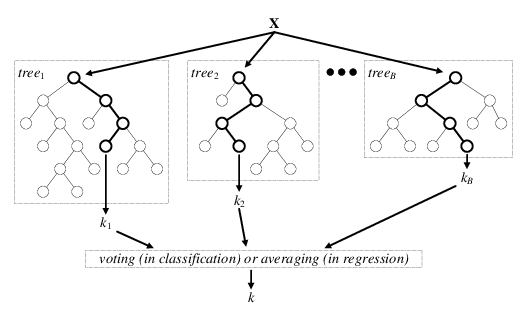
\includegraphics[width=400px]{random_forest.png}
		\caption{Random forest}
	\end{figure}
	Random forests or random decision forests are an ensemble learning method for classification, regression and other tasks, that operate by constructing a multitude of decision trees at training time and outputting the class that is the mode of the classes (classification) or mean prediction (regression) of the individual trees. Random decision forests correct for decision trees' habit of overfitting to their training set.
	\par Random forest algorithms are a part of ensemble learning, the machine learning technique which does not rely only one type of learning methods. This is what makes ensemble learning more robust and generalized as compared to other machine learning algorithms. Most common form of random forest algorithms use multiple decision trees, i.e. random forest are based on decision trees. Random forests create multiple decision trees and merges them together to get a more accurate and stable prediction.	
\end{enumerate}

\newpage
\section{Observations and Results}
\par According to the pre-designed workflow, we used four above mentioned algorithms for training and testing of diabetes and tested cross-validation for test data 20\%, 30\% and 40\% respectively.
\par Below images show the accuracy outputs of all four algorithms in all 20, 30 and 40\% test datasets.

\begin{figure}[h]
	\centering
	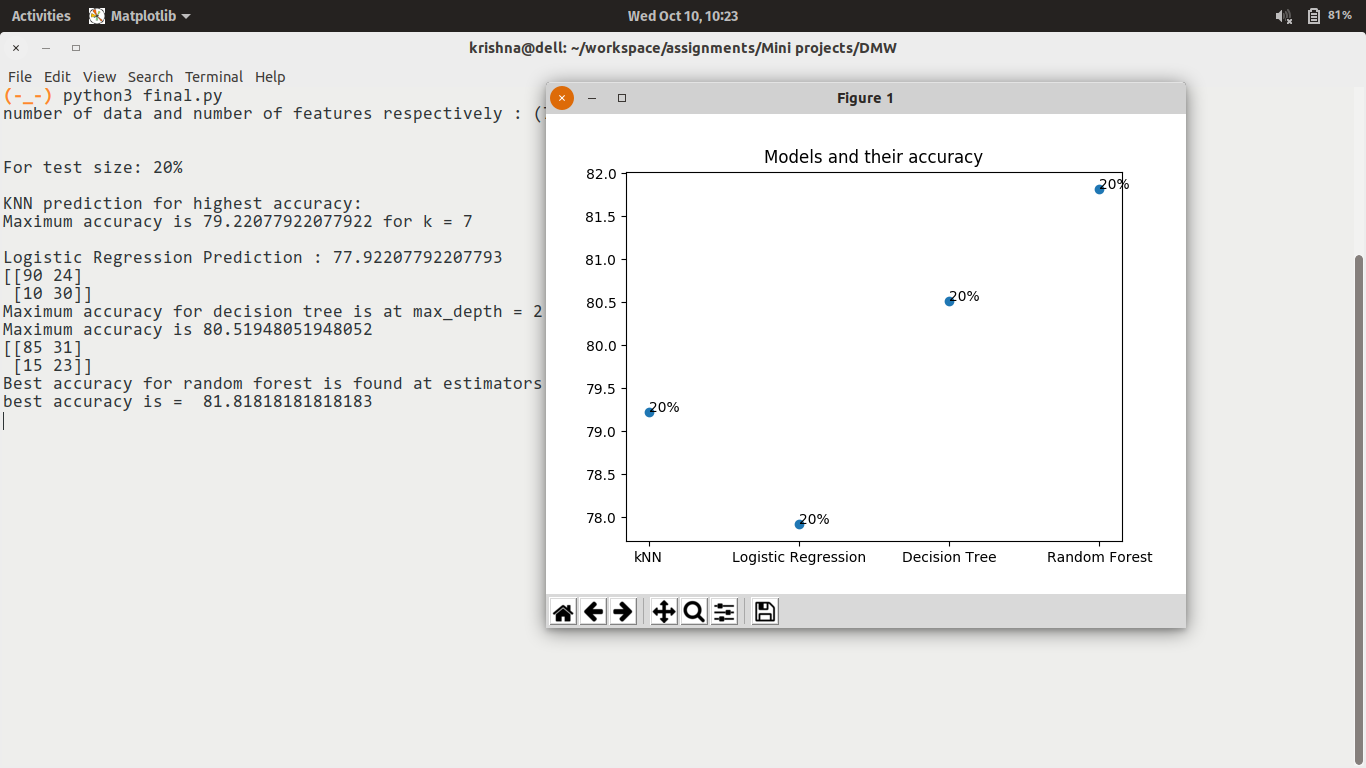
\includegraphics[width=300px]{output_20.png}
	\caption{accuracy for test = 20\%}
\end{figure}

\begin{figure}
	\centering
	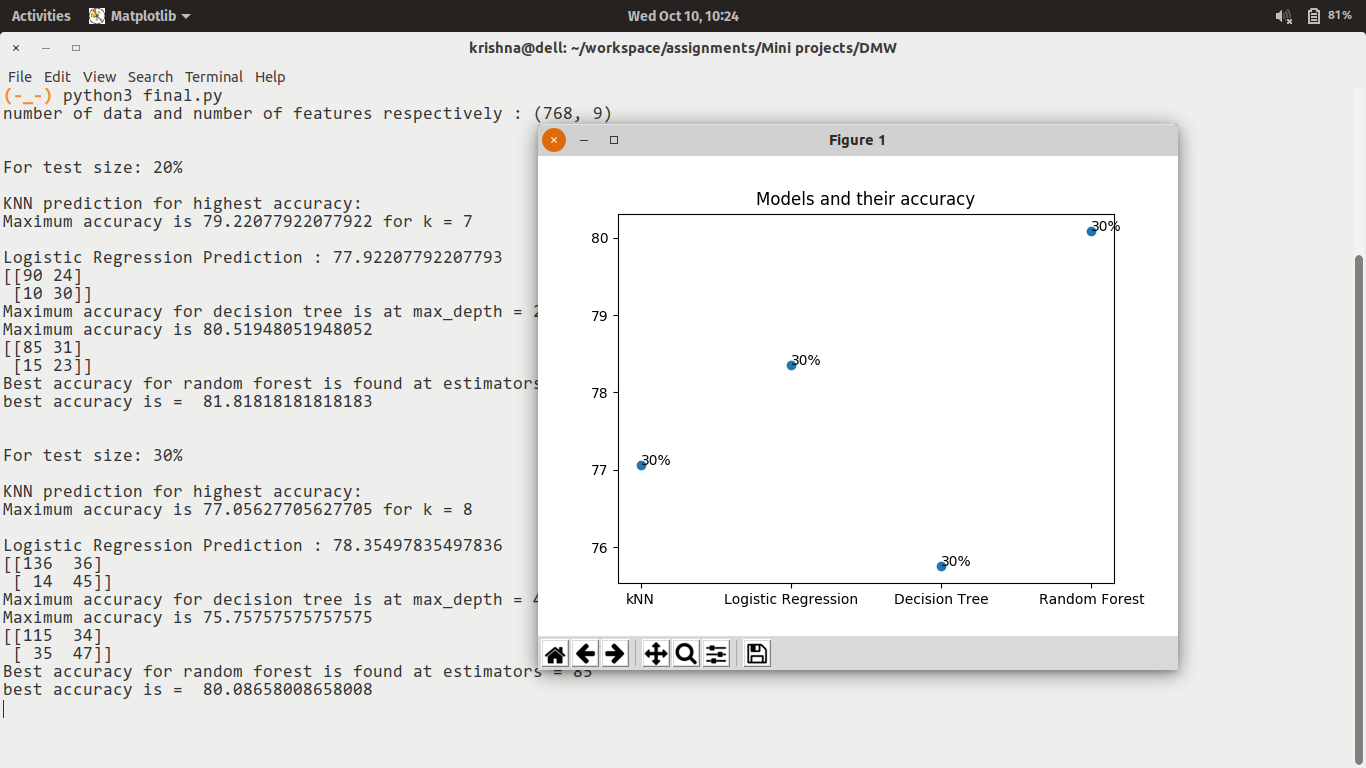
\includegraphics[width=350px]{output_30.png}
	\caption{accuracy for test = 30\%}
\end{figure}

\begin{figure}
	\centering
	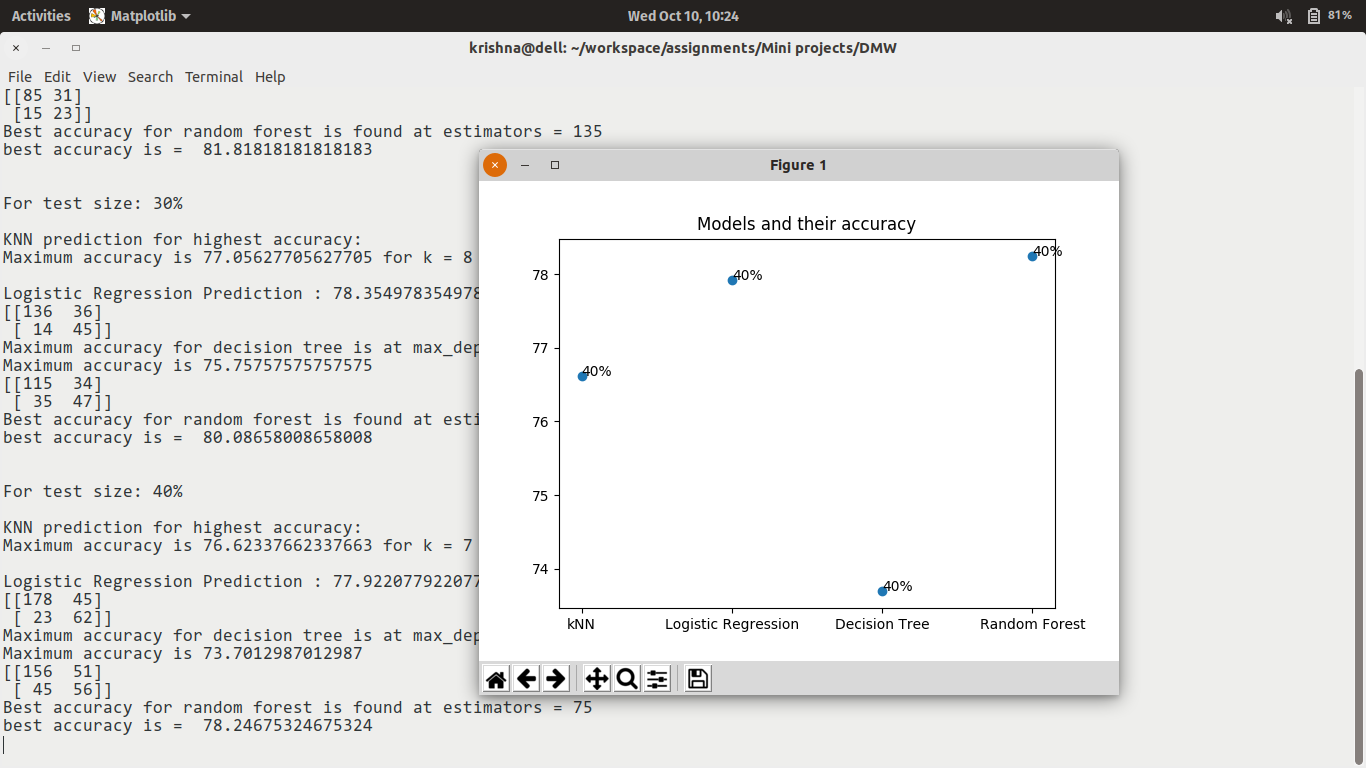
\includegraphics[width=350px]{output_40.png}
	\caption{accuracy for test = 40\%}
\end{figure}
\newpage
By above observations, it is found that \textbf{random forest} algorithm outperforms all other algorithms in every case, having a consistent accuracy of around 81\%.
\section{Conclusion}
\par Hence, we learned and implemented various machine learning algorithms and performed data preprocessing, training and testing of algorithms and analyzed the results of accuracy of 4 machine learning algorithms including decision tree, logistic regression, kNN and random forest algorithms.
\end{document}